\documentclass{article}
\usepackage{graphicx}% Required for inserting images
\usepackage{lindrew}
\usepackage{pdfpages}
\usepackage[shortlabels]{enumitem}
\usepackage{matlab-prettifier}
\usepackage{algorithm}
\usepackage{algpseudocode}

\title{ACM 104 Problem Set 5}
\author{Amitesh Pandey}
\date{November 2024}
\begin{document}
\maketitle
\section*{Problem 2: Hermite Polynomials}
\emph{Solution. }In a similar fashion to the Legendre polynomials, the Hermite polynomials may be calculated as following with respect to the given inner product,

\begin{equation*}
\begin{aligned}
&\begin{aligned}
    h_{0}(x) = 1
\end{aligned}\\
&\begin{aligned}
    h_{1}(x) &= x - \frac{\langle x, 1\rangle}{||1||^2} = x - 0 = x
\end{aligned}\\
&\begin{aligned}
h_2(x) & =x^2-\frac{\left\langle x^2, 1\right\rangle}{\|1\|^2}-\frac{\left\langle x^2, x\right\rangle}{\|x\|^2} \cdot x \\
& =x^2-\frac{\sqrt{2 \pi}}{\sqrt{2 \pi}} =x^2-1
\end{aligned}\\
&\begin{aligned}
h_3(x) & =x^3-\frac{\left\langle x^3, 1\right\rangle}{\|1\|^2}-\frac{\left\langle x^3, x\right\rangle}{\|x\|^2} \cdot x-\frac{\left\langle x^3, x^2-1\right\rangle}{\left\|x^2-1\right\|^2} \cdot\left(x^2-1\right) \\
& =x^3-\frac{3 \sqrt{2 \pi}}{\sqrt{2 \pi}} \cdot x =x^3-3 x
\end{aligned}\\
&\begin{aligned}
h_4(x) & =x^4-\frac{\left\langle x^4, 1\right\rangle}{\|1\|^2}-\frac{\left\langle x^4, x\right\rangle}{\|x\|^2} \cdot x-\frac{\left\langle x^4, x^2-1\right\rangle}{\left\|x^2-1\right\|^2} \cdot\left(x^2-1\right)\\
&-\frac{\left\langle x^4, x^3-3 x\right\rangle}{\left\|x^3-3 x\right\|^2} \cdot\left(x^3-3 x\right) \\
& =x^4-\frac{3 \sqrt{2 \pi}}{\sqrt{2 \pi}}-\frac{12 \sqrt{2 \pi}}{2 \sqrt{2 \pi}} \cdot\left(x^2-1\right) \\
& =x^4-6 x^2+3
\end{aligned}
\end{aligned}
\end{equation*}
\newpage
\section*{Problem 3: Orthogonal Compliments}
\emph{Solution. }For $W_{1}^{\perp}$, conveniently note that vectors that are  perpendicular to both $x$ and $y$ will naturally be perpendicular to all possible linear combinations of $x$ and $y$, which means, the span of $v_1 \times v_2$ will be complimenting $W$ under this product. More specifically, we will have
\begin{equation*}
    W_{1}^{\perp} = \text{span}\{v_1\times v_2\} = \text{span}\left\{\begin{pmatrix}
        1 \\
        2 \\
        3
    \end{pmatrix} \times \begin{pmatrix}
        2\\
        0\\
        1
    \end{pmatrix}\right\} = \text{span}\left\{\begin{pmatrix}
        2\\
        5\\
        -4
    \end{pmatrix}\right\}
\end{equation*}
For $W_{2}^{\perp}$, note that the basis $u$ will be such that $\langle v_{1}, u\rangle = \langle v_2, u\rangle$. For general $u$, 
\begin{equation*}
    \langle v_{1}, u\rangle = \langle [1, 2, 3]^{T}, u\rangle = u_{x} + 4u_{y} + 9u_{z}
\end{equation*}
Similarly for the second vector, we have
\begin{equation*}
    \langle v_{2}, u \rangle = \langle [2, 0, 1]^{T}, u\rangle = 2u_{x} + u_{z}
\end{equation*}
So we need $u_{x}, u_{y}, u_{z}$ that simultaneously satisfy
\begin{align*}
    u_{x}  + 4u_{y} + 9u_{z} &= 0\\
    2u_{x} + u_{z} &= 0
\end{align*}
In terms of $u_{z}$, we simply the above expressions to get $u_{x} = \frac{-3}{2}u_{z}$ and $u_{y} = \frac{-15}{8}u_{z}$. This means
\begin{equation*}
    W_{2}^{\perp} = \text{span}\left\{\begin{pmatrix}
        \frac{-3u_{z}}{2}\\
        \frac{-15u_{z}}{8}\\
        u_{z}
    \end{pmatrix}\right\} = \text{span}\left\{\begin{pmatrix}
        \frac{-3}{2}\\
        \frac{-15}{8}\\
        1
    \end{pmatrix}\right\}
\end{equation*}
\section*{Problem 4: Complete Matrices}
\emph{Solution. }The matrix $A$ is complete if and only if all eigenvalues have algebraic and geometric multiplicities of 1. First consider for an eigenvalue $\text{det}(A - \lambda I) = 0$. We essentially have
\begin{equation*}
    \text{det}(A - \lambda I) = \text{det}\begin{pmatrix}
        -\lambda & 0 & -1 \\
        0 & 1-\lambda & 0 \\
        1 & 0 & -\lambda
    \end{pmatrix} = 0
\end{equation*}
This implies $-\lambda^{3} + \lambda^{2} - \lambda + 1 = 0$. By trial and error, we find $\lambda \neq 0$. However $\lambda = 1$ is a root. Then factoring $\lambda - 1$ out, we obtain the other coefficient as
\begin{equation*}
    (\lambda - 1)(-\lambda^{2} - 1) = 0
\end{equation*}
This implies $\lambda = \pm i$. At this point, note that all three roots (eigenvalues) have algebraic multiplicities of 1.
\newpage
\noindent{Now}, we check if all three eigenvalues have geometric multiplicity of 1.
\begin{enumerate}
    \item When $\lambda =1$, 
    \begin{equation*}
        Av = \lambda v \implies Av = v \implies v = \langle 0, k , 0\rangle
    \end{equation*}
    \item When $\lambda = i$, 
    \begin{equation*}
        Av = \lambda v \implies Av= iv\implies = v = \langle ki, 0, k\rangle
    \end{equation*}
    \item When $\lambda = i$, 
    \begin{equation*}
        Av = \lambda v \implies Av = -iv \implies v = \langle -ki, 0, k\rangle
    \end{equation*}
\end{enumerate}
In each of the cases, the basis for the subspace spanned by $v$ is defined completely using only 1 vector (setting $k = 1$ for example). Since the dimension is 1, in each of the cases, the span of the eigenvector has geometric multiplicity 1, so $A$ is therefore complete.
\section*{Problem 5}
\emph{Solution. }(a) From the definition of the Gershgorin disk, we have
\begin{align*}
    \mathcal{D}_{1} &= \left\{z \in \mathbb{C} \ \left| \ |z - b_{11}| \leq \sum_{j\neq 1}|b_{1j}|\right\} = \{z \in \mathbb{C} \ | \ |z| \leq 1\}\\
    \mathcal{D}_{2} &= \left\{z \in \mathbb{C} \ \left| \ |z - b_{22}| \leq \sum_{j\neq 2}|b_{2j}|\right\} = \{z \in \mathbb{C} \ | \ |z - 1| \leq 1\}\\
    \mathcal{D}_{3} &= \left\{z \in \mathbb{C} \ \left| \ |z - b_{33}| \leq \sum_{j\neq 3}|b_{3j}|\right\} = \{z \in \mathbb{C} \ | \ |z - 1| \leq 1\}
\end{align*}
This makes it clear that there will be two discs, centered at $(0,0)$ and $(1, 0)$. The domain will be as follows:
\begin{figure}[htp]
    \centering
    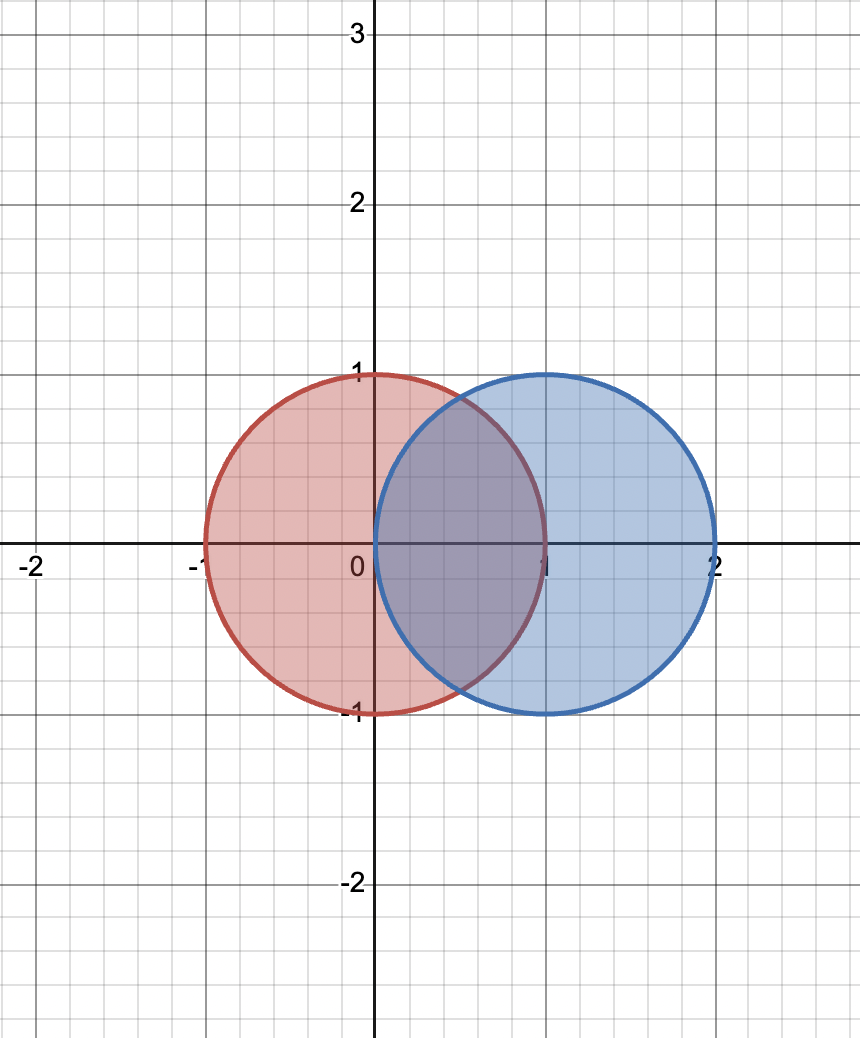
\includegraphics[width=2in]{img1.png}
    \label{fig:galaxy}
\end{figure}
\newpage
\noindent{(b)} First of all, from Gershgorin's Theorem, we know that $\text{spec}(A) \subset D_{A}$. Note for all $\lambda$ such that $\text{det}(A - \lambda I) =0$, then we have $\text{det}((A - \lambda I)^{T}) = 0 \implies \text{det}(A^{T} - \lambda I) = 0$. But all $\lambda$ that satisfy this form $D_{A^{T}}$. This implies $\text{spec}(A) \subset D_{A^{T}}$. Since $\text{spec}(A) \subset D_{A}$ and $\text{spec}(A) \subset D_{A^{T}}$, we trivially have $\text{spec}(A) \subset D_{A}^{*}$. \\\\
(c) For the refined domain, let's first find the domain for $B^{T}$. 
\begin{equation*}
    B^{T} = \begin{pmatrix}
        0 &0& 0\\
        1 &1 &-1\\
        0 &1 &1
    \end{pmatrix}
\end{equation*}
Then we simply have
\begin{align*}
    \mathcal{D}_{1} &= \{z \in \mathbb{C} \ | \ |z| \leq 0 \}\\
    \mathcal{D}_{2} &= \{z \in \mathbb{C} \ | \ |z - 1| \leq 2 \} \\
    \mathcal{D}_{3} &= \{z \in \mathbb{C} \ | \ |z - 1| \leq 1\}
\end{align*}
We can ignore $\mathcal{D}_{1}$ (because it's a point that's anyways contained in a disk for $B$). Note that $\mathcal{D}_{3}$ is also identical to a disk for $B$. For $\mathcal{D}_{2}$, we have a circle centered at (1,0) with radius 2. This circle encapsulates all remaining disks of $B$, so the domain $D_{B}^{*}$ finally is:
\begin{figure}[htp]
    \centering
    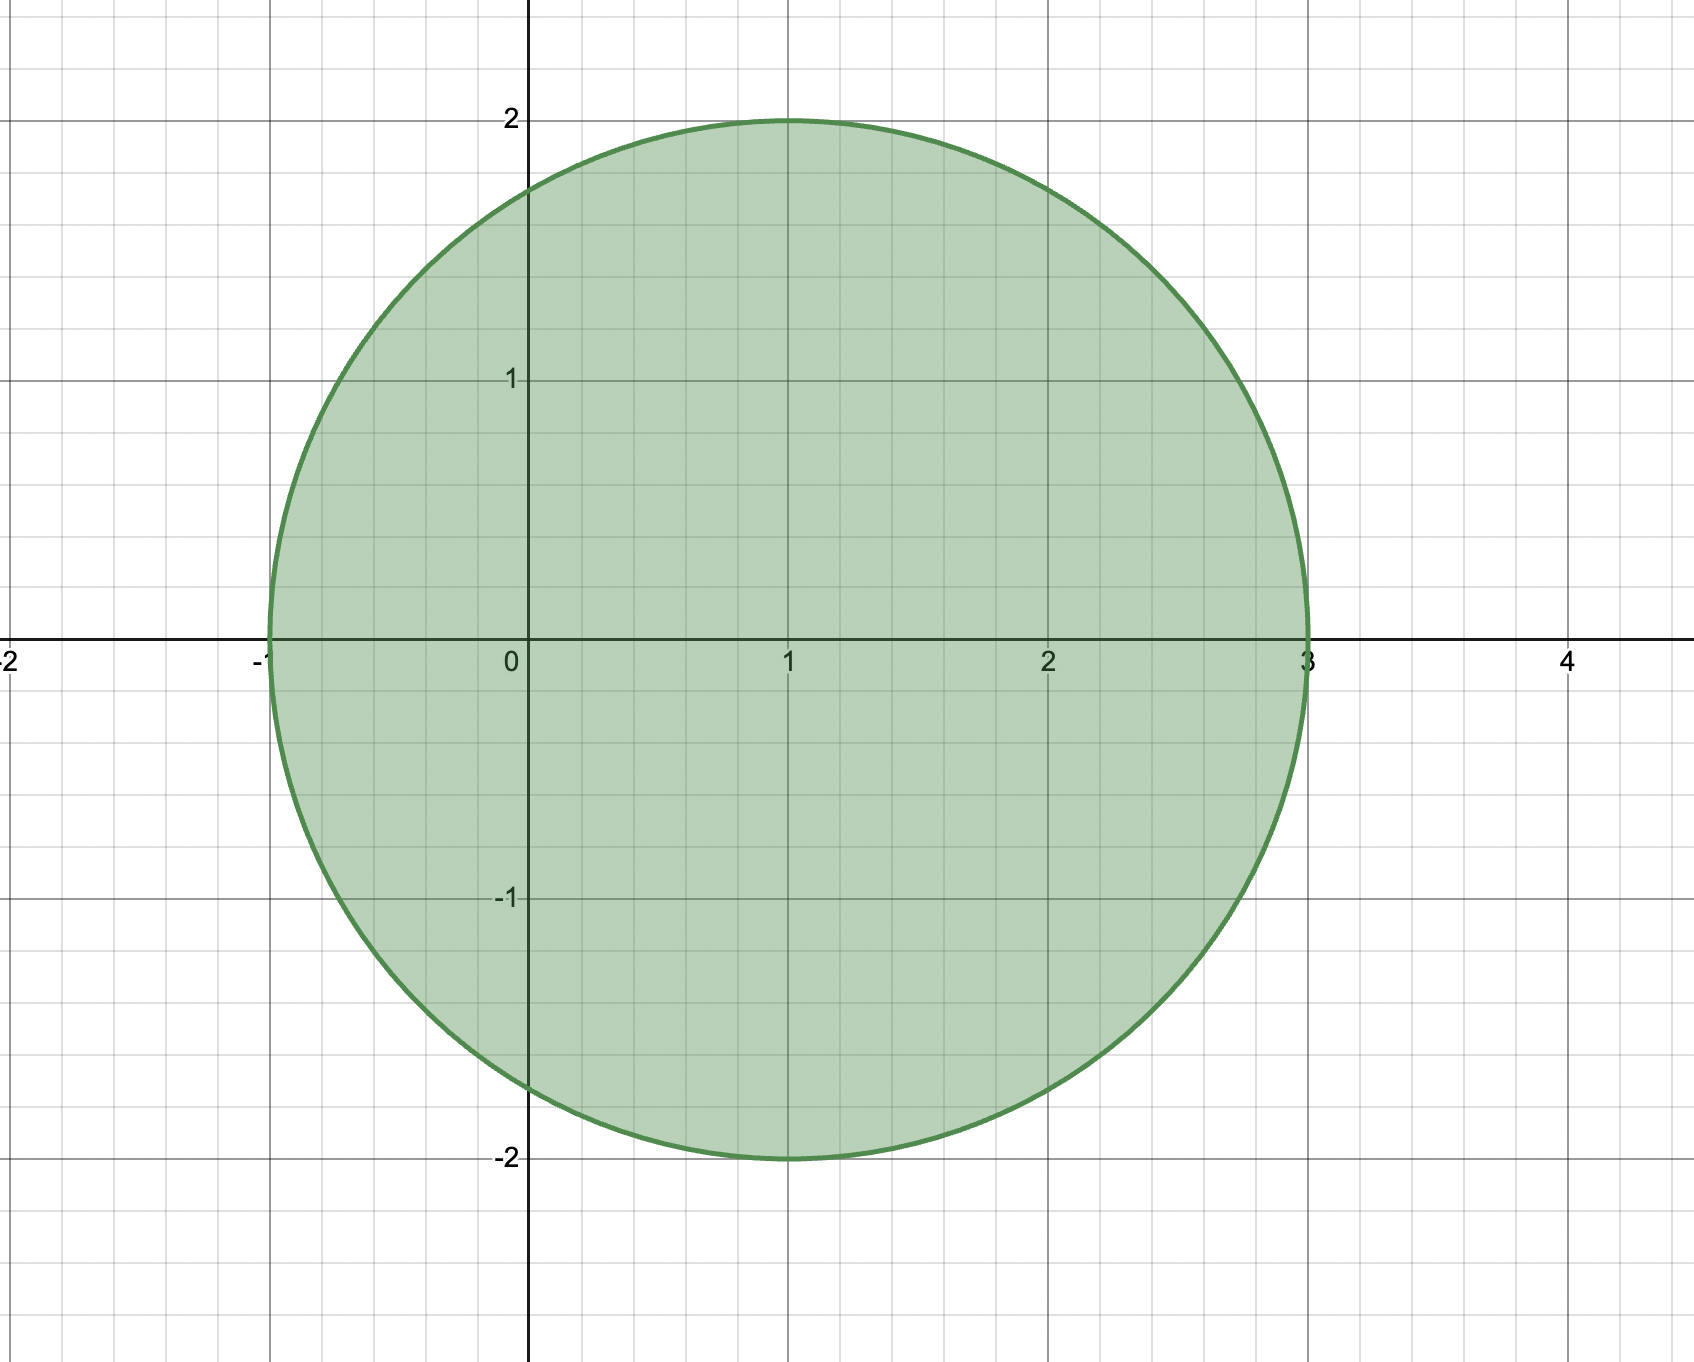
\includegraphics[width=2in]{img2.png}
    \label{fig:galaxy}
\end{figure}\\\\
(d) The eigenvalues satisfy $\text{det}(B - \lambda I) = 0$. We have
\begin{equation*}
    \det (B - \lambda I) = \det \begin{pmatrix}
        -\lambda & 1 & 0\\
        0 & 1 - \lambda & 1\\
        0 & -1  & 1 - \lambda
    \end{pmatrix} = -\lambda ((1-\lambda)^2 + 1)
\end{equation*}
This makes it clear (by observation) that the eigenvalues are $\lambda = 0, 1 - i, 1 + i$. Clearly all of them lie in the green disk above, so they do belong to $D_{B}^{*}$. \\\\
(e) Consider the matrix 
\begin{equation*}
    B = \begin{pmatrix}
        0 & 3\\
        7 & 1
    \end{pmatrix}
\end{equation*}
This matrix has $\mathcal{D}_{1} = \{z \in \mathbb{C} \ | \ |z| \leq 3\}$ and $\mathcal{D}_{2} = \{z \in \mathbb{C} \ | \ |z-1| \leq 7\}$. Clearly the point (0,0) is contained in the first disc, so the domain $\mathcal{D}_{1}\cup \mathcal{D}_{2}$ contains zero and it's also easy to see that the determinant is not zero. 
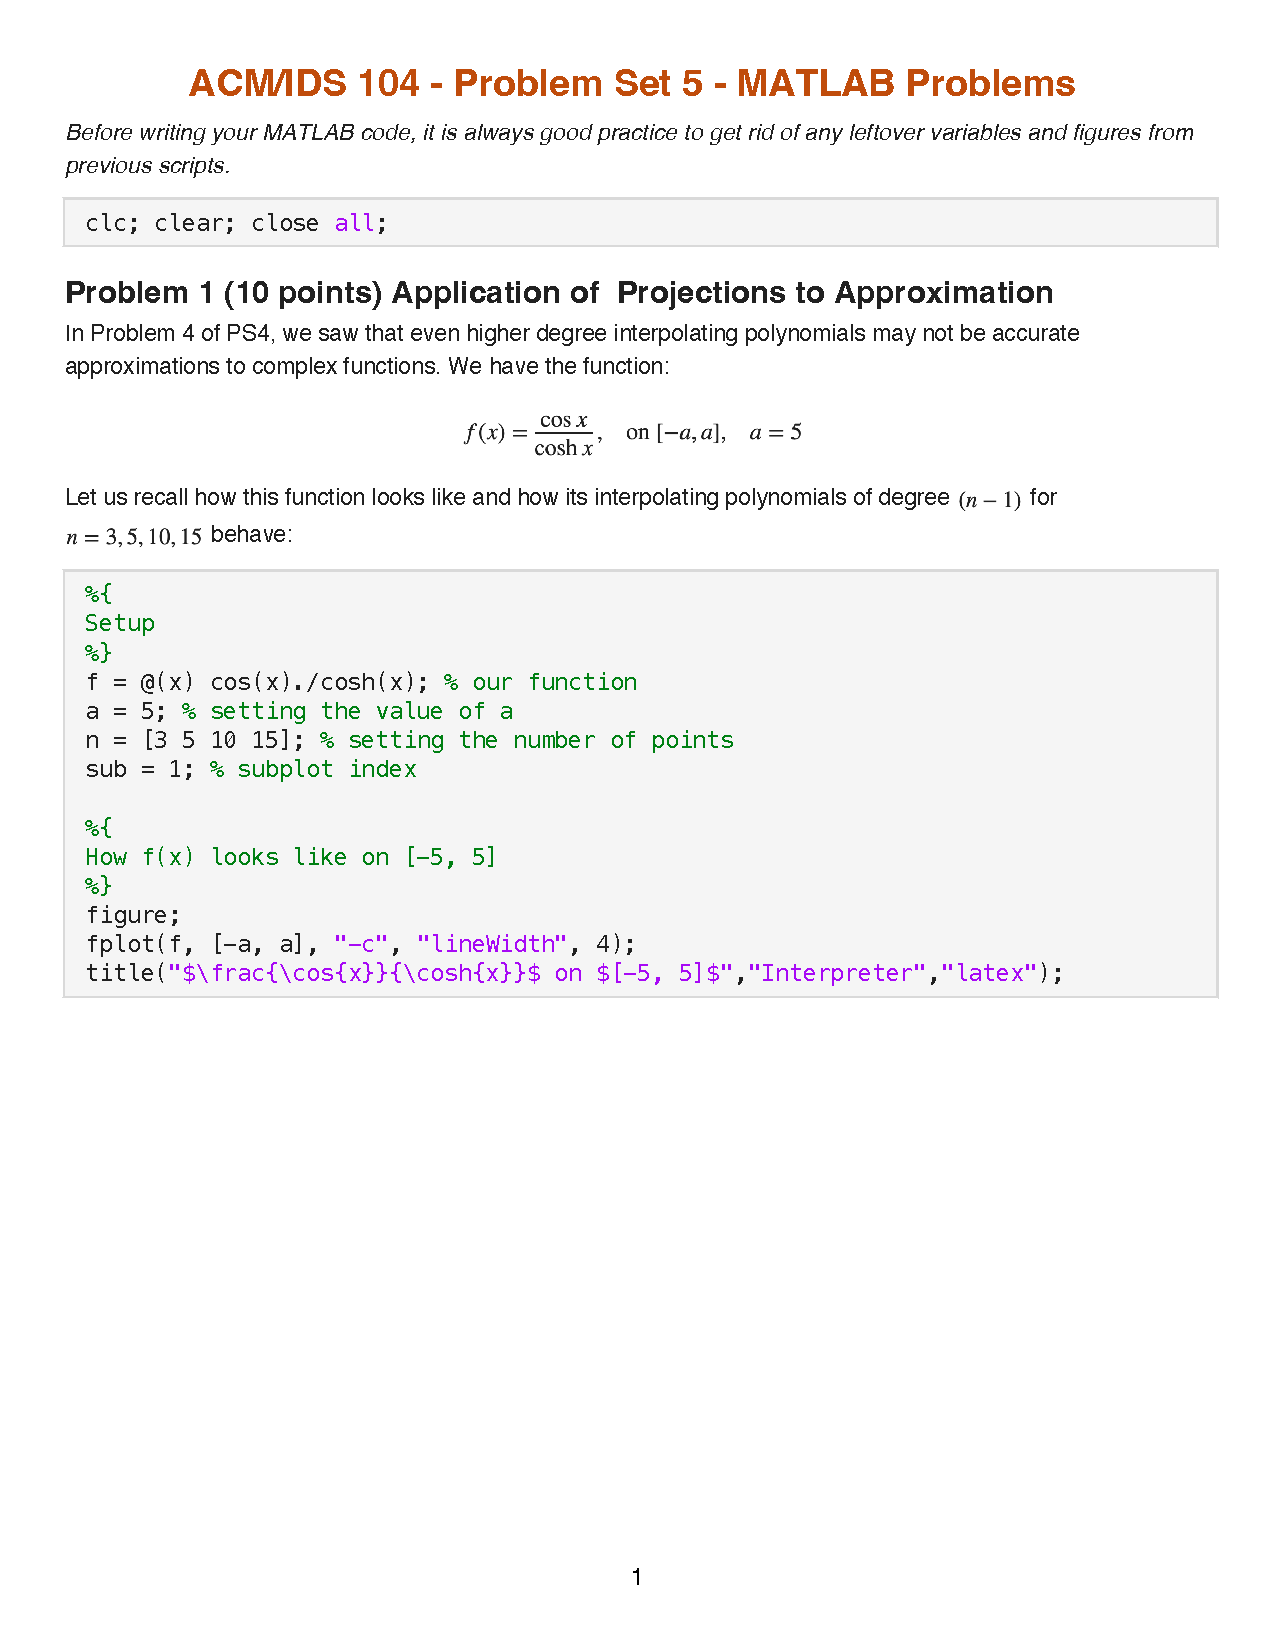
\includepdf[pages=-]{PS5matlab.pdf}
\end{document}
